% =====================================================================
%  MIPS Multi-Cycle CPU -- Innovation Fair Bangladesh poster
%  30 in x 72 in portrait banner.
%
%  Build (run twice):
%      pdflatex -interaction=nonstopmode poster.tex
%
%  Content is derived from README.md and ARCHITECTURE.md.
%  Figures come from ../docs/diagrams/ (see poster/README.md).
%
%  NOTE ON PAGE SIZE: tikzposter hard-codes a0paper in its option list
%  and derives every block/column width from \textwidth at class-load
%  time, so a custom paper size must be applied AFTER the class and the
%  derived widths recomputed -- see the block below.
%
%  NOTE ON VERTICAL FIT: tikzposter spreads rows to fill the page height
%  when the content fits, and silently overflows (clipping the last rows)
%  when it does not -- it does NOT warn. After editing, always re-check
%  that the last block still appears (see poster/README.md).
% =====================================================================
\documentclass[
  25pt,
  margin=0.8in,
  innermargin=0.6in,
  colspace=0.8in,
  blockverticalspace=0.32in
]{tikzposter}

\geometry{paperwidth=30in,paperheight=72in}
\makeatletter
\setlength{\TP@visibletextwidth}{\textwidth-2\TP@innermargin}
\setlength{\TP@visibletextheight}{\textheight-2\TP@innermargin}
\makeatother

% --- Type scale ------------------------------------------------------
% The 25pt class option loads a0size.sty, which sets a very large scale
% (\large = 29.86pt) -- and tikzposter renders every block BODY at \large.
% At that size this much content does not fit the 72in height. Rescale
% the display sizes; block titles stay chunky, body text stays readable.
\renewcommand{\normalsize}{\fontsize{19.5}{24}\selectfont}
\renewcommand{\large}{\fontsize{21}{26}\selectfont}
\renewcommand{\Large}{\fontsize{26}{31.5}\selectfont}
\renewcommand{\LARGE}{\fontsize{31}{37}\selectfont}
\renewcommand{\huge}{\fontsize{37}{44}\selectfont}
\renewcommand{\Huge}{\fontsize{57}{65}\selectfont}
\renewcommand{\small}{\fontsize{17.5}{21.5}\selectfont}
\renewcommand{\footnotesize}{\fontsize{15.5}{19}\selectfont}
\renewcommand{\scriptsize}{\fontsize{13.5}{16.5}\selectfont}
\renewcommand{\tiny}{\fontsize{12}{14.5}\selectfont}
\normalsize

\usepackage[T1]{fontenc}
\usepackage{helvet}
\renewcommand{\familydefault}{\sfdefault}
\usepackage{graphicx}
\usepackage{booktabs}
\usepackage{array}
\usepackage{tabularx}
\usepackage{colortbl}
\usepackage{amsmath,amssymb}

\graphicspath{{../docs/diagrams/}}

% Drop tikzposter's "LaTeX TikZposter" corner watermark -- it is noise on
% a printed poster.
\tikzposterlatexaffectionproofoff

\usetheme{Simple}

% The Simple theme uses the Minimal block style, whose defaults are
% titleinnersep=1cm and bodyinnersep=1cm. Across ~11 blocks that padding
% alone eats roughly 9in of the 72in height, so trim it.
\useblockstyle[titleinnersep=0.6cm, bodyinnersep=0.45cm]{Minimal}

% --- Palette ---------------------------------------------------------
% Mirrors the colour key published in ARCHITECTURE.md, so the poster and
% the diagrams read as one artefact.
\definecolor{cStorage}{HTML}{E8890C}
\definecolor{cCompute}{HTML}{1971C2}
\definecolor{cMemory}{HTML}{2F9E44}
\definecolor{cControl}{HTML}{7048E8}
\definecolor{cClock}{HTML}{868E96}
\definecolor{cIO}{HTML}{E03131}
\definecolor{fClock}{HTML}{F1F3F5}

\colorlet{backgroundcolor}{fClock}
\colorlet{framecolor}{cClock}
\colorlet{titlebgcolor}{white}
\colorlet{titlefgcolor}{black}
\colorlet{blockbodybgcolor}{white}
\colorlet{blockbodyfgcolor}{black}
\colorlet{blocktitlefgcolor}{white}
\colorlet{notefrcolor}{cCompute}

% Blocks take no colour keys, so the accent is swapped in before each
% \block call. (nb: not \accent -- that is a LaTeX primitive.)
\newcommand{\accentcolor}[1]{\colorlet{blocktitlebgcolor}{#1}}

\setlength{\parindent}{0pt}
\renewcommand{\arraystretch}{1.15}
\newcommand{\hdr}[1]{\textbf{#1}}

\title{MIPS Multi-Cycle CPU}
\author{A 17-instruction Verilog softcore on the Altera Cyclone~IV~E FPGA}
\institute{
  EP4CE6E22C8 \ \textbullet\ \ Quartus Prime 25.1std Lite
  \ \textbullet\ \ 12.5\,MHz core (50\,MHz\,$\div$\,4)
  \ \textbullet\ \ 6{,}150 / 6{,}272 LEs (98\,\%)
  \ \textbullet\ \ timing closed, $+$12.558\,ns slack
}

\begin{document}
\maketitle

% =====================================================================
% ROW 1 -- At a Glance  |  System Overview
% =====================================================================
\begin{columns}
\column{0.40}
\accentcolor{cControl}
\block{At a Glance}{
  \renewcommand{\arraystretch}{1.35}
  \begin{tabular}{@{}r@{\hspace{0.9em}}l@{}}
  {\LARGE\bfseries 17}     & instructions in the ISA \\
  {\LARGE\bfseries 10}     & control-FSM states \\
  {\LARGE\bfseries 12.5}   & MHz core clock (50\,MHz\,$\div$\,4) \\
  {\LARGE\bfseries 98\,\%} & logic fit --- 6{,}150 / 6{,}272 LEs \\
  {\LARGE\bfseries 5}      & ISSP debug cores, 2{,}232 bits \\
  {\LARGE\bfseries 4{,}096} & $\times$ 32 on-chip instruction memory \\
  {\LARGE\bfseries 16}     & M9K blocks for \texttt{imem} (30 available) \\
  \end{tabular}

  \vspace{0.8em}
  A \textbf{single shared datapath}, reused 3--5 times per instruction by
  an FSM, instead of one long combinational path. On-chip instruction and
  data memory, memory-mapped I/O, a UART program loader and five
  in-system probes make it a complete, debuggable softcore.

  \vspace{0.6em}
  Setup slack on \texttt{clk} is \textbf{+12.558\,ns} against the 20\,ns
  period, so the design closes timing at 50\,MHz with room to spare. The
  large register count is dominated by the ISSP probe shadow registers
  (4\,$\times$\,480 + 312 bits) plus the 32\,$\times$\,32-bit register
  file.
}

\column{0.60}
\accentcolor{cClock}
\block{System Overview --- Board Level}{
  \begin{center}
  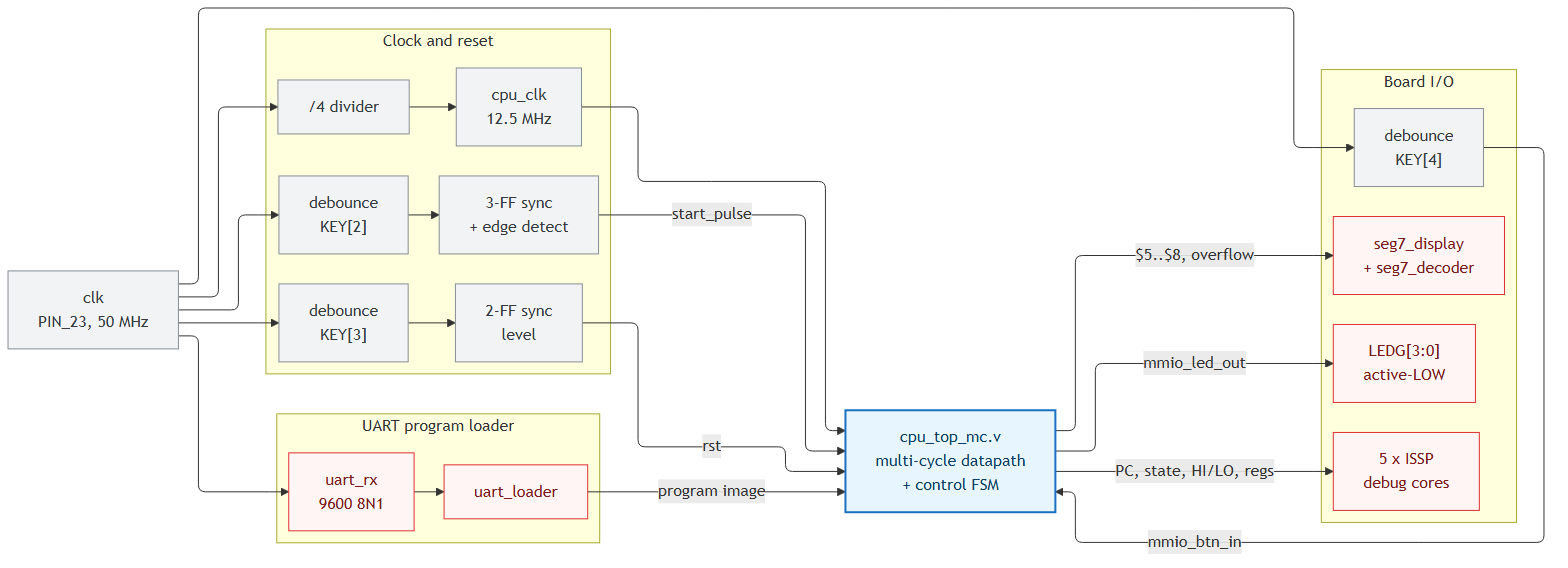
\includegraphics[width=\linewidth]{01-1-system-overview-board-level.png}
  \end{center}
  \vspace{0.2em}
  \texttt{top\_cpu\_mc.v} is the top-level entity. It owns every
  board-specific concern --- pin wiring, the clock divider, button
  debouncing and the JTAG debug probes --- and wraps the CPU, which runs
  on the divided clock.

  \textbf{Two clock domains.} The debouncers, the UART receiver, the
  loader and \texttt{imem}'s write port all run on the raw 50\,MHz clock,
  because their timing is calibrated in real milliseconds or baud
  periods. The CPU itself runs on \texttt{cpu\_clk} at 12.5\,MHz. Only
  \textbf{two} signals cross between the domains --- \texttt{rst} and
  \texttt{start\_pulse} --- and both are synchronized first. \texttt{start}
  is edge-detected \emph{inside} the slow domain on purpose: a
  single-cycle pulse generated at 50\,MHz could be too narrow for a
  12.5\,MHz clock to ever sample.
}
\end{columns}

% =====================================================================
% ROW 2 -- Instruction Set (full width, split into two half-tables)
% =====================================================================
\begin{columns}
\column{1}
\accentcolor{cCompute}
\block{Instruction Set --- 17 Instructions Decoded}{
  \begin{center}
  \renewcommand{\arraystretch}{1.12}
  \begin{minipage}[t]{0.47\linewidth}
  \centering
  \begin{tabular}{@{}llll@{}}
  \toprule
  \hdr{Mnemonic} & \hdr{Format} & \hdr{Opcode} & \hdr{Funct} \\
  \midrule
  \texttt{ADD}  & R & \texttt{000000} & \texttt{100000} \\
  \texttt{SUB}  & R & \texttt{000000} & \texttt{100010} \\
  \texttt{AND}  & R & \texttt{000000} & \texttt{100100} \\
  \texttt{OR}   & R & \texttt{000000} & \texttt{100101} \\
  \texttt{SLT}  & R & \texttt{000000} & \texttt{101010} \\
  \texttt{MULT} & R & \texttt{000000} & \texttt{011000} \\
  \texttt{DIV}  & R & \texttt{000000} & \texttt{011010} \\
  \texttt{MFHI} & R & \texttt{000000} & \texttt{010000} \\
  \texttt{MFLO} & R & \texttt{000000} & \texttt{010010} \\
  \texttt{JR}   & R & \texttt{000000} & \texttt{001000} \\
  \bottomrule
  \end{tabular}
  \end{minipage}\hfill
  \begin{minipage}[t]{0.47\linewidth}
  \centering
  \begin{tabular}{@{}llll@{}}
  \toprule
  \hdr{Mnemonic} & \hdr{Format} & \hdr{Opcode} & \hdr{Funct} \\
  \midrule
  \texttt{ADDI} & I & \texttt{001000} & --- \\
  \texttt{LW}   & I & \texttt{100011} & --- \\
  \texttt{SW}   & I & \texttt{101011} & --- \\
  \texttt{BEQ}  & I & \texttt{000100} & --- \\
  \texttt{BNE}  & I & \texttt{000101} & --- \\
  \texttt{JAL}  & J & \texttt{000011} & --- \\
  \texttt{HALT} & --- & \texttt{111111} & --- \\[0.2em]
  \multicolumn{4}{@{}l@{}}{\textit{Formats:} R = register, I = immediate, J = jump.} \\[0.2em]
  \multicolumn{4}{@{}l@{}}{\textit{Syntax:} \texttt{ADD \$rd,\$rs,\$rt} \ \textbullet\ \ \texttt{LW \$rt,off(\$rs)}} \\
  \multicolumn{4}{@{}l@{}}{\phantom{\textit{Syntax:}} \texttt{BEQ \$rs,\$rt,label} \ \textbullet\ \ \texttt{JAL label}} \\
  \bottomrule
  \end{tabular}
  \end{minipage}
  \end{center}

  \vspace{0.5em}
  \textbf{Encoding notes.} Branches are PC-relative: \texttt{offset} $=$
  \texttt{label} $-$ (\texttt{addr}$+$1), a 16-bit signed field
  range-checked by the assembler. \texttt{JAL} is \emph{not} standard
  pseudo-direct addressing --- the assembler emits an absolute target and
  the hardware reads only \texttt{ir\_reg[11:0]}, a 12-bit absolute target
  that is valid because \texttt{imem} is 4{,}096 words. \texttt{HALT} is a
  project-specific opcode. \texttt{MULT}/\texttt{DIV} take no
  \texttt{rd}: results land in HI/LO and are read out with
  \texttt{MFHI}/\texttt{MFLO}.
}
\end{columns}

% =====================================================================
% ROW 3 -- The Datapath  |  Compute Units
% =====================================================================
\begin{columns}
\column{0.55}
\accentcolor{cStorage}
\block{The Datapath --- Structural Data Flow}{
  \begin{center}
  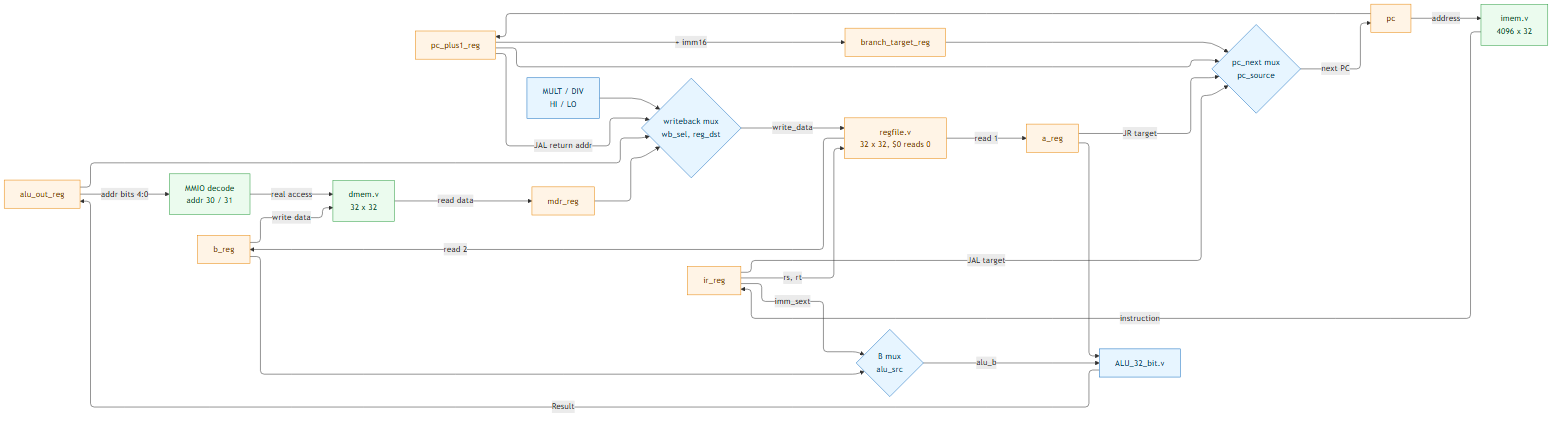
\includegraphics[width=\linewidth]{02-2-1-data-flow.png}
  \end{center}
  \vspace{0.2em}
  The 18 control signals are deliberately omitted from the diagram: they
  fan out from a single FSM node, and drawing each as an edge turns the
  figure into an unreadable web.

  \vspace{0.3em}
  $\bullet$ \textbf{Decode happens off \texttt{ir\_reg}}, not the
  \texttt{imem} output. \texttt{pc} is frozen for the whole instruction, so
  the instruction fields are latched and stay valid through ID/EX/MEM/WB.

  $\bullet$ \textbf{The PC updates exactly once per instruction, during
  EX}, for \emph{every} instruction type. \texttt{pc\_source} selects the
  next value from four candidates: fall-through, branch target, JAL
  target, JR target.

  $\bullet$ \textbf{Write-back} selects between \texttt{alu\_out\_reg},
  \texttt{mdr\_reg}, HI and LO; the destination is \texttt{rd},
  \texttt{rt} or \texttt{\$31}.

  \vspace{0.3em}
  Cross-cycle registers hold partial results between cycles, so control
  only decides \emph{which} register latches on a given clock edge.
}

\column{0.45}
\accentcolor{cCompute}
\block{Compute Units --- ALU and MULT/DIV}{
  \textbf{ALU.} 31 identical \texttt{alu\_1bit} slices plus an
  \texttt{alu\_1Xbit} MSB slice that exports its raw sum bit for SLT
  (Patterson \& Hennessy style).

  \vspace{0.5em}
  \begin{center}
  \renewcommand{\arraystretch}{1.12}
  \begin{tabular}{@{}ll@{}}
  \toprule
  \texttt{Op[3:0]} & \textbf{Operation} \\
  \midrule
  \texttt{0000} & AND \\
  \texttt{0001} & OR \\
  \texttt{0010} & ADD \\
  \texttt{0110} & SUB (\texttt{A + \textasciitilde{}B + 1}) \\
  \texttt{0111} & SLT \\
  \texttt{1100} & NOR \\
  \bottomrule
  \end{tabular}
  \end{center}
  \vspace{0.4em}
  Flags: \texttt{Ov} $=$ \texttt{Carry[30]} $\oplus$ \texttt{Cout}
  (signed overflow), and \texttt{LT} $=$ \texttt{Ov} $\oplus$
  \texttt{Set}, which corrects the SLT sign when overflow occurred.

  \vspace{0.7em}
  \textbf{MULT / DIV} share one 64-bit working register and one
  32-iteration state, \texttt{MD\_LOOP}. Sharing is safe because
  \texttt{ir\_reg} is stable, so only one can ever be in flight.

  \vspace{0.3em}
  $\bullet$ \textbf{MULT} --- shift-add: if the low half's LSB is set, add
  the multiplicand into the high half, then shift the whole register
  right.\par
  $\bullet$ \textbf{DIV} --- restoring division: shift left, subtract the
  divisor from the high half, then either restore (shift in \texttt{0}) or
  keep (shift in \texttt{1}).\par
  $\bullet$ \textbf{Result} --- after 32 steps the quotient sits in the
  low half and the remainder in the high half, exactly the MIPS LO/HI
  convention, so no reshuffling is needed. The remainder follows the
  \emph{dividend's} sign, as in real MIPS.
}
\end{columns}

% =====================================================================
% ROW 4 -- Instruction Timing  |  Memory, MMIO and Board I/O
% =====================================================================
\begin{columns}
\column{0.52}
\accentcolor{cClock}
\block{Instruction Timing}{
  \begin{center}
  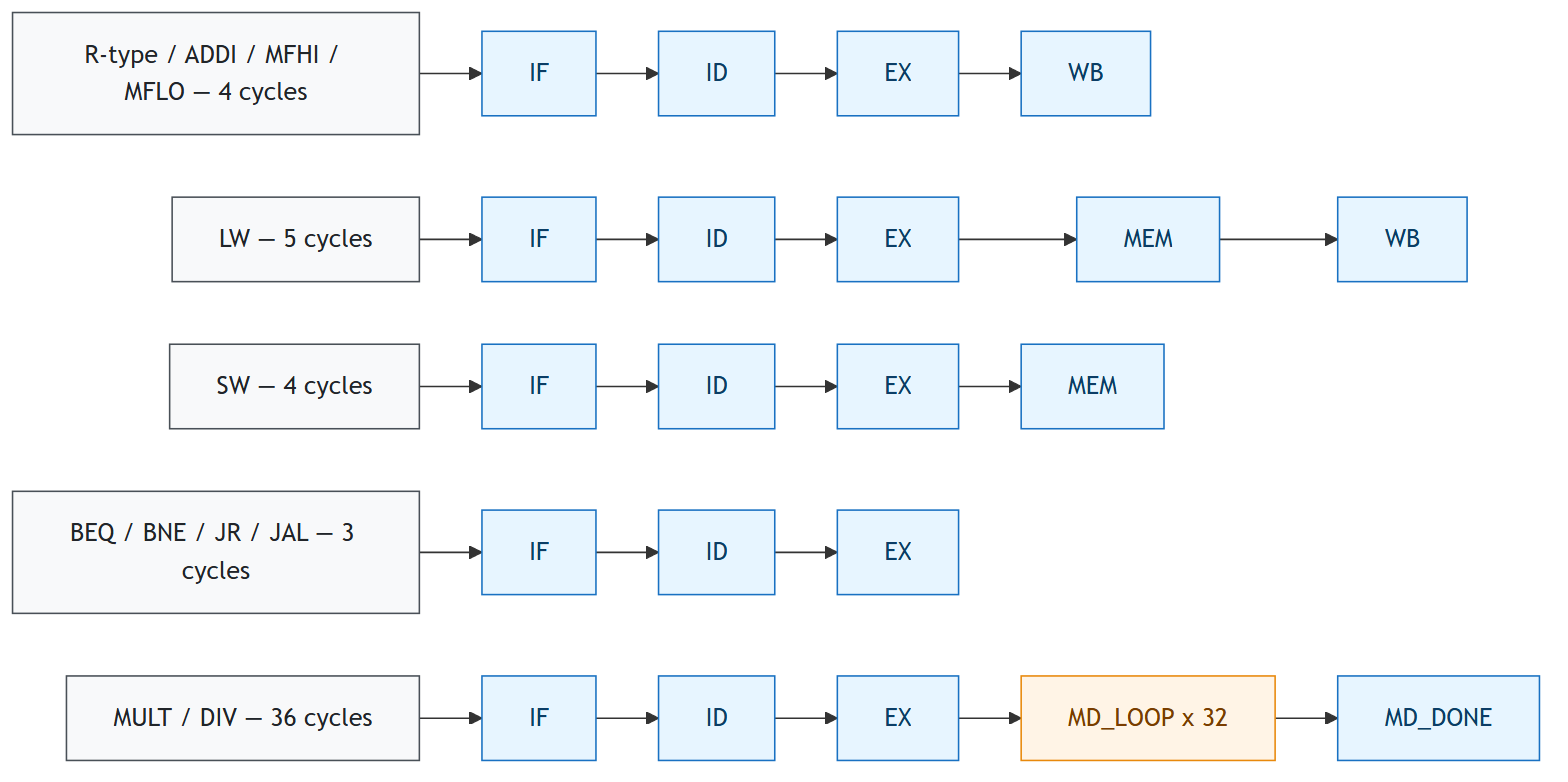
\includegraphics[height=3.85in]{10-10-instruction-timing.png}
  \end{center}
  \vspace{0.2em}
  Cycle counts are on \texttt{cpu\_clk} at 12.5\,MHz, so a plain ALU
  instruction takes \textbf{320\,ns}. \texttt{IDLE} is \emph{not} counted
  --- it is visited once after reset, then never again.

  \vspace{0.5em}
  \begin{center}
  \renewcommand{\arraystretch}{1.12}
  \begin{tabularx}{\linewidth}{@{}l>{\raggedright\arraybackslash}Xc@{}}
  \toprule
  \textbf{Instruction} & \textbf{States} & \textbf{Cycles} \\
  \midrule
  ADD / SUB / AND / OR / SLT & IF, ID, EX, WB & 4 \\
  ADDI, MFHI, MFLO           & IF, ID, EX, WB & 4 \\
  LW                         & IF, ID, EX, MEM, WB & 5 \\
  SW                         & IF, ID, EX, MEM & 4 \\
  BEQ / BNE                  & IF, ID, EX & 3 \\
  JR / JAL                   & IF, ID, EX & 3 \\
  MULT / DIV                 & IF, ID, EX, $32\times$ MD\_LOOP, MD\_DONE & \textbf{36} \\
  HALT / illegal opcode      & IF, ID, EX $\to$ stuck & 3 \\
  \bottomrule
  \end{tabularx}
  \end{center}
}

\column{0.48}
\accentcolor{cMemory}
\block{Memory, Memory-Mapped I/O and Board I/O}{
  \texttt{dmem} keeps a 5-bit address, so only the low 5 bits of a
  computed address are used. Two addresses are intercepted \textbf{before}
  reaching \texttt{dmem.v}, leaving that module completely unmodified.

  \vspace{0.5em}
  \begin{center}
  \renewcommand{\arraystretch}{1.12}
  \begin{tabularx}{\linewidth}{@{}cl>{\raggedright\arraybackslash}X@{}}
  \toprule
  \textbf{Address} & \textbf{LW} & \textbf{SW} \\
  \midrule
  0--29 & ordinary read & ordinary write \\
  30    & \textbf{MMIO} $\to$ \texttt{\{31'b0,KEY[4]\}} & ordinary write to \texttt{mem[30]} \\
  31    & ordinary read of \texttt{mem[31]} & \textbf{MMIO} $\to$ \texttt{led\_reg[3:0]} \\
  \bottomrule
  \end{tabularx}
  \end{center}
  \vspace{0.3em}
  The asymmetry means \texttt{mem[30]} is unreachable via \texttt{LW} and
  \texttt{mem[31]} via \texttt{SW}, but each stays reachable in the other
  direction. The LEDs are physically \textbf{active-LOW}; the inversion is
  done at the pin so the core stays board-agnostic.

  \vspace{0.7em}
  \hdr{Board I/O}
  \vspace{0.4em}
  \begin{center}
  \renewcommand{\arraystretch}{1.12}
  \begin{tabular}{@{}ll@{}}
  \toprule
  \textbf{Signal} & \textbf{Role} \\
  \midrule
  \texttt{KEY[2]}   & \textbf{Start / run} --- one press runs the whole program \\
  \texttt{KEY[3]}   & \textbf{Reset} --- held as a level, not a pulse \\
  \texttt{KEY[1:0]} & Selects which of \texttt{\$5}--\texttt{\$8} is displayed \\
  \texttt{KEY[4]}   & MMIO input button (read from address 30) \\
  7-seg DP          & Lights when the sticky overflow flag is set \\
  \texttt{LEDG[3:0]} & MMIO output (active-LOW) \\
  UART              & 8N1, 9600 baud program loader \\
  \bottomrule
  \end{tabular}
  \end{center}
}
\end{columns}

% =====================================================================
% ROW 5 -- Control FSM  |  ISSP Debug
% =====================================================================
\begin{columns}
\column{0.46}
\accentcolor{cControl}
\block{Multi-Cycle Control FSM}{
  \begin{center}
  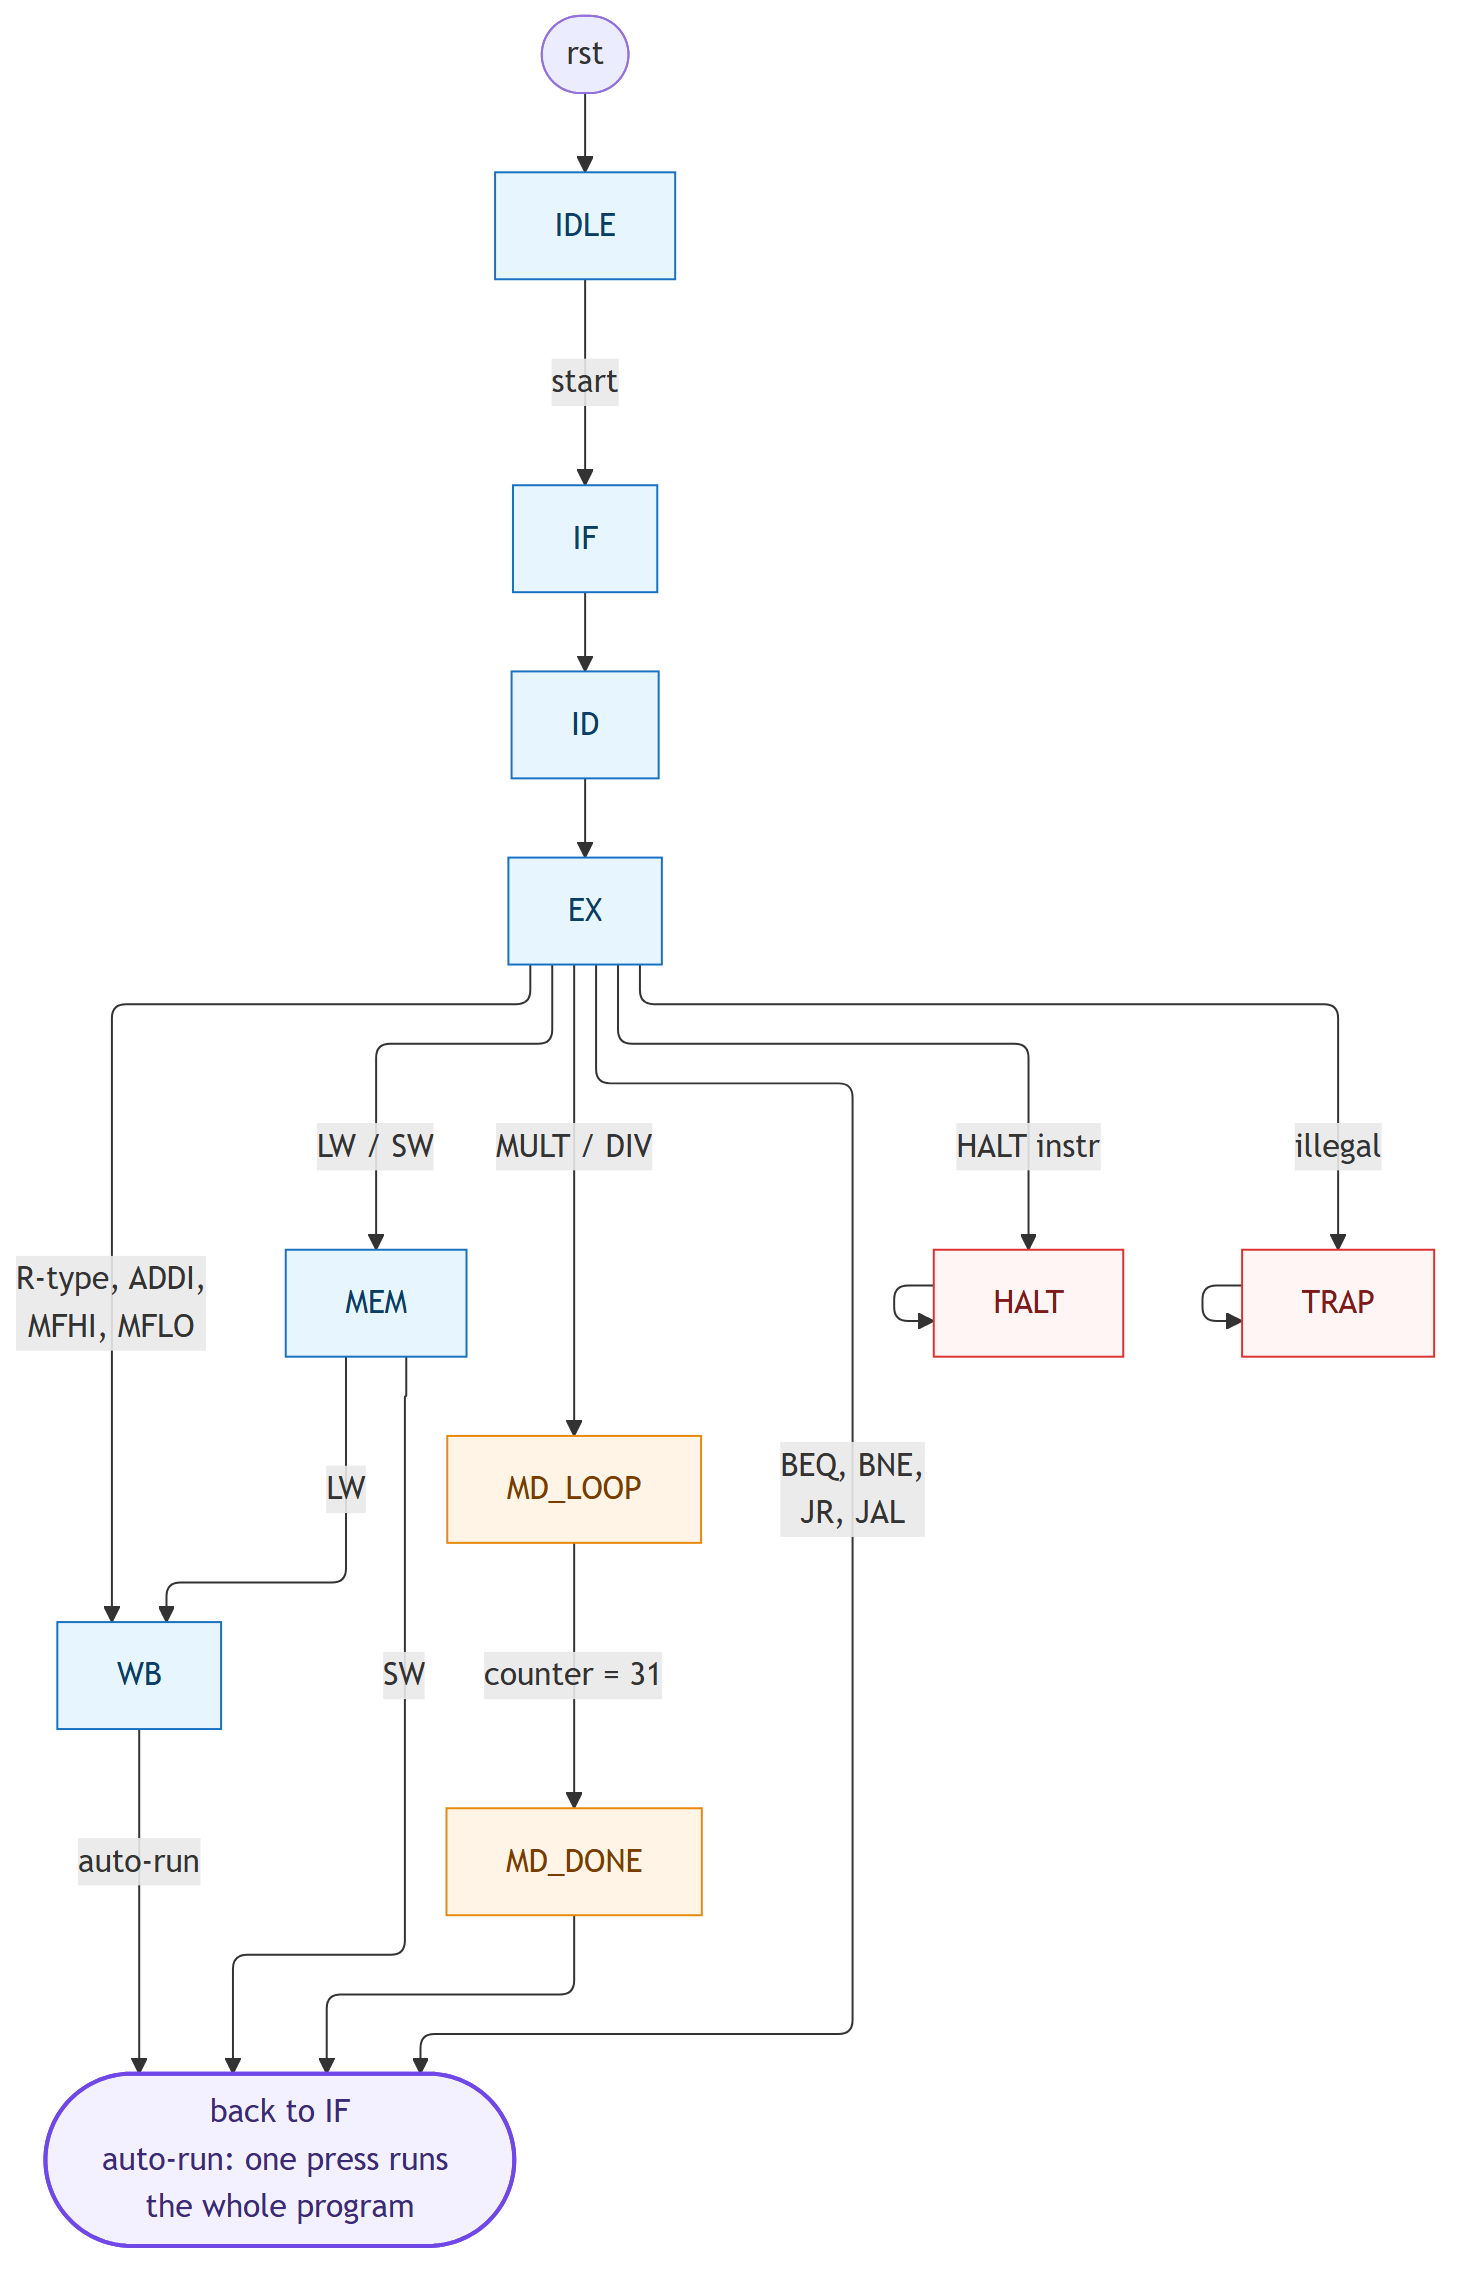
\includegraphics[height=4.15in]{06-6-2-state-diagram.png}
  \end{center}
  \vspace{0.3em}
  \textbf{Auto-run.} Every instruction's terminal transition points back
  to \texttt{IF}, not \texttt{IDLE}, so a single button press free-runs
  the \emph{entire} program. \texttt{IDLE} is entered exactly once, after
  reset.

  \vspace{0.3em}
  \textbf{Absorbing states.} \texttt{TRAP} (illegal opcode) and
  \texttt{HALT} (explicit stop) are permanent --- only \texttt{rst} leaves
  them. The sticky \texttt{illegal\_opcode} flag latches when \texttt{TRAP}
  is entered, so the flag and ``the FSM is stuck'' always agree.

  \vspace{0.3em}
  The control unit holds \textbf{no data at all} --- only the current
  state. It decodes the latched instruction and asserts per-state pulses:
  \textbf{11} latch enables and \textbf{6} mux selects out, \textbf{4}
  status signals in.

  \vspace{0.5em}
  \begin{center}
  \renewcommand{\arraystretch}{1.1}
  \begin{tabularx}{\linewidth}{@{}ll>{\raggedright\arraybackslash}X@{}}
  \toprule
  \textbf{State} & \textbf{Enc.} & \textbf{Next state} \\
  \midrule
  \texttt{IDLE}    & \texttt{0} & \texttt{IF} if start, else \texttt{IDLE} \\
  \texttt{IF}      & \texttt{1} & \texttt{ID} \\
  \texttt{ID}      & \texttt{2} & \texttt{EX} \\
  \texttt{EX}      & \texttt{3} & \texttt{TRAP} / \texttt{HALT} / \texttt{MD\_LOOP} / \texttt{MEM} / \texttt{WB} / \texttt{IF} \\
  \texttt{MEM}     & \texttt{4} & \texttt{WB} if LW, else \texttt{IF} \\
  \texttt{WB}      & \texttt{5} & \texttt{IF} \\
  \texttt{TRAP}    & \texttt{6} & \texttt{TRAP} (absorbing) \\
  \texttt{MD\_LOOP} & \texttt{7} & \texttt{MD\_DONE} if counter $=31$, else itself \\
  \texttt{MD\_DONE} & \texttt{8} & \texttt{IF} \\
  \texttt{HALT}    & \texttt{9} & \texttt{HALT} (absorbing) \\
  \bottomrule
  \end{tabularx}
  \end{center}
}

\column{0.54}
\accentcolor{cIO}
\block{Debug --- In-System Source and Probe Cores}{
  \begin{center}
  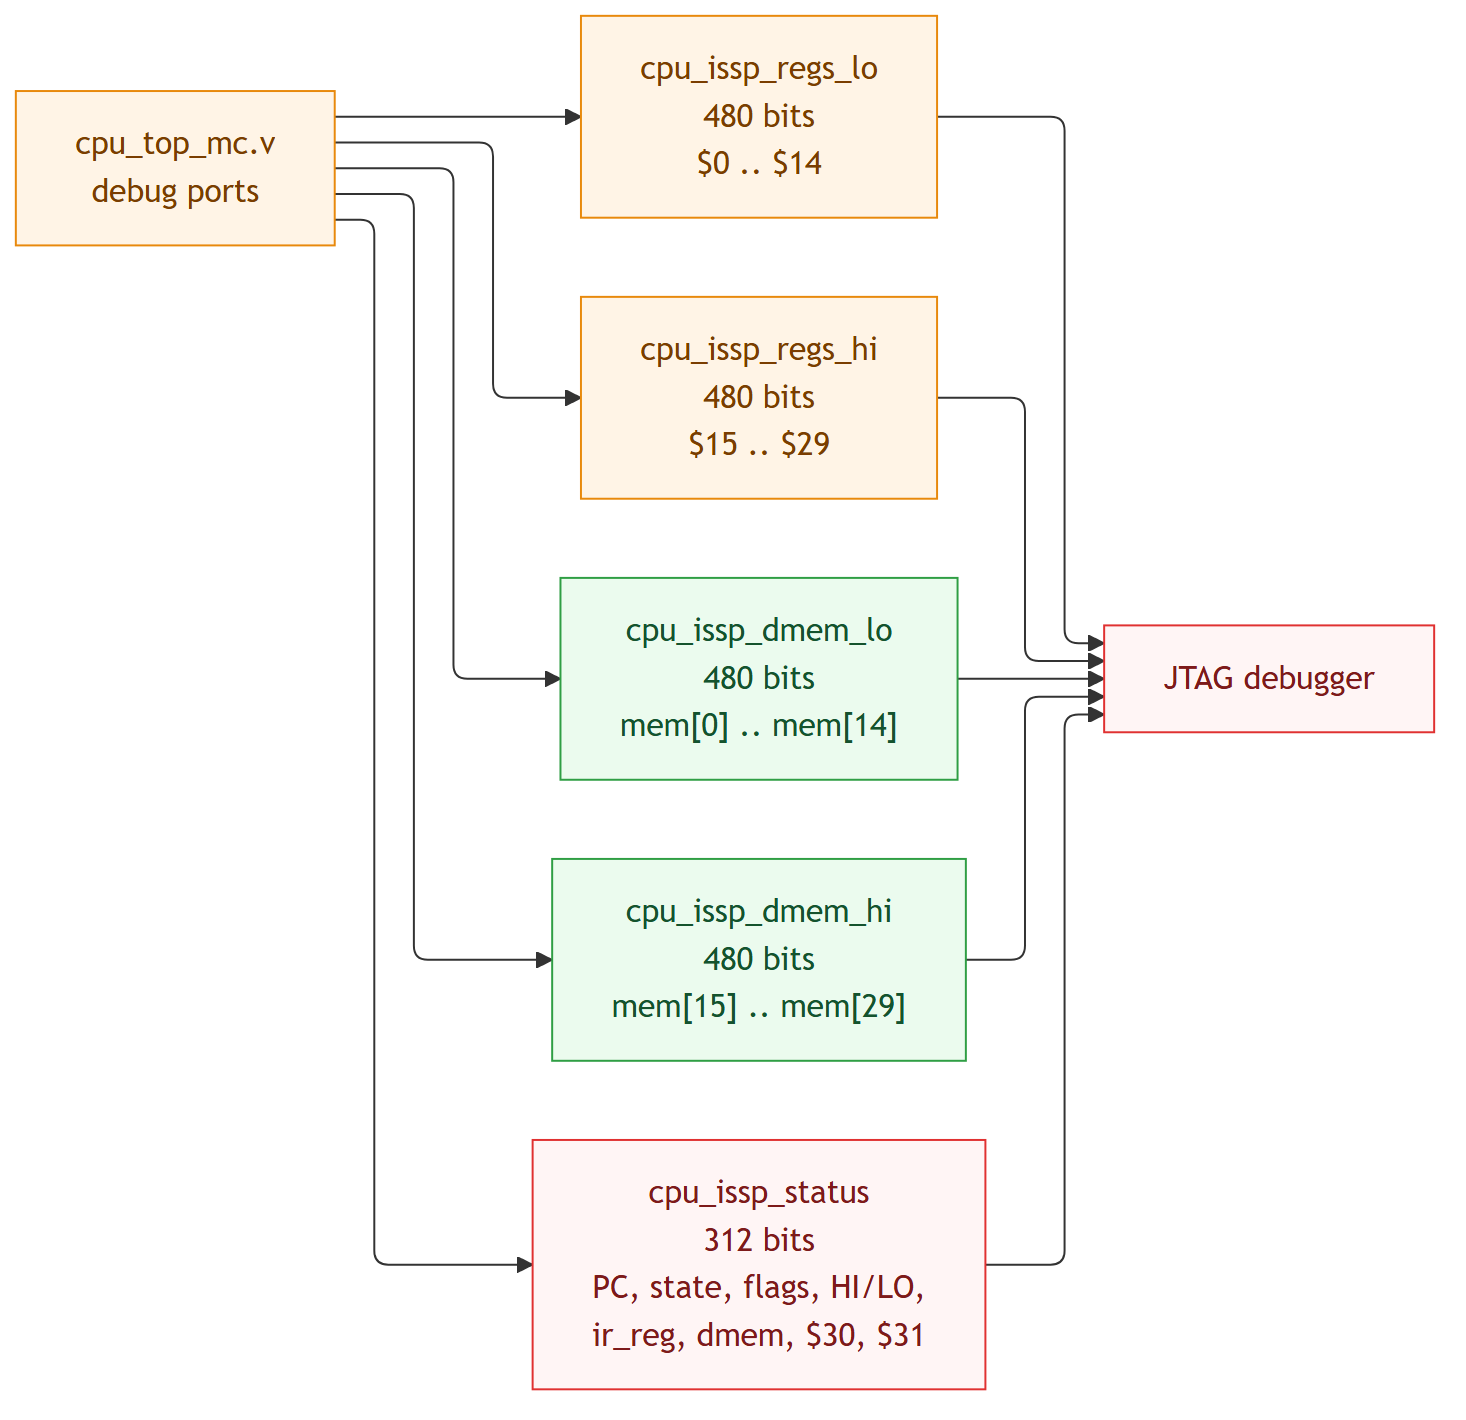
\includegraphics[height=4.15in]{09-9-issp-debug-probe-layout.png}
  \end{center}
  \vspace{0.3em}
  Five \texttt{altera\_in\_system\_sources\_probes} cores are clocked from
  the JTAG domain. Word $n$ within an instance occupies bits
  \texttt{[32n+31 : 32n]}, with no gaps.

  \vspace{0.5em}
  \begin{center}
  \renewcommand{\arraystretch}{1.12}
  \begin{tabularx}{\linewidth}{@{}lc>{\raggedright\arraybackslash}X@{}}
  \toprule
  \textbf{Core} & \textbf{Width} & \textbf{Contents} \\
  \midrule
  \texttt{\_regs\_lo}  & 480 & \texttt{\$0}--\texttt{\$14} \\
  \texttt{\_regs\_hi}  & 480 & \texttt{\$15}--\texttt{\$29} \\
  \texttt{\_dmem\_lo}  & 480 & \texttt{mem[0]}--\texttt{mem[14]} \\
  \texttt{\_dmem\_hi}  & 480 & \texttt{mem[15]}--\texttt{mem[29]} \\
  \texttt{\_status}    & 312 & PC, FSM state, sticky flags, HI/LO, \texttt{ir\_reg}, \texttt{\$30}, \texttt{\$31}, \texttt{mem[30]}, \texttt{mem[31]} \\
  \bottomrule
  \end{tabularx}
  \end{center}
  \vspace{0.3em}
  Core names are all prefixed \texttt{cpu\_issp}.

  \vspace{0.5em}
  \textbf{Why five cores?} \texttt{ALTSOURCE\_PROBE} has a hard
  \textbf{511-bit \texttt{PROBE\_WIDTH} limit} --- 16 words would be 512
  bits and is rejected. Each core therefore carries 15 words (480 bits),
  and the four leftovers are folded into the status core, which has
  headroom.

  \vspace{0.5em}
  \textbf{Debugging tips.} Watch the FSM state field to see exactly which
  cycle is executing. State \texttt{6} means an illegal instruction was
  decoded --- freeze and inspect \texttt{ir\_reg}. State \texttt{9} means
  the program hit its \texttt{HALT}. If results look wrong, check the
  sticky \textbf{overflow} flag before suspecting the arithmetic.
}
\end{columns}

% =====================================================================
% ROW 6 -- Build and run  |  Design journey
% =====================================================================
\begin{columns}
\column{0.5}
\accentcolor{cCompute}
\block{Build, Load and Run}{
  \textbf{1. Write} a program in the subset assembly syntax.\par
  \textbf{2. Assemble:} \texttt{python3 assembler.py program.asm} emits
  \texttt{program.hex} (4{,}096 lines) and \texttt{data.hex} (32 lines),
  both zero-padded to full depth.\par
  \textbf{3. Compile} in Quartus Prime (25.1std Lite): Analysis \&
  Synthesis $\to$ Fitter $\to$ Assembler $\to$ TimeQuest.\par
  \textbf{4. Program} the device with
  \texttt{output\_files/Mips\_Multi\_Cycle\_Cpu.sof} over JTAG.\par
  \textbf{5. Run} --- press \texttt{KEY[2]} once; \texttt{KEY[3]} resets.

  \vspace{0.5em}
  The assembler is a single-file Python 3 script with no dependencies. It
  appends a trailing \texttt{HALT} automatically if the source does not
  end with one --- important, because in auto-run mode the FSM never
  returns to \texttt{IDLE}, so a program without a stop would run off the
  end into the zero padding and land in \texttt{TRAP}.

  \vspace{0.55em}
  \hdr{Quick reference}
  \vspace{0.4em}
  \begin{center}
  \renewcommand{\arraystretch}{1.2}
  \begin{tabularx}{\linewidth}{@{}l>{\raggedright\arraybackslash}X@{}}
  \toprule
  Assemble & \texttt{python3 assembler.py program.asm} \\
  Build & \texttt{quartus\_sh --flow compile Mips\_Multi\_Cycle\_Cpu} \\
  Program & \texttt{Mips\_Multi\_Cycle\_Cpu.sof} via JTAG \\
  Run & \texttt{KEY[2]} --- one press $=$ whole program \\
  Reset & \texttt{KEY[3]} \\
  Display & \texttt{KEY[1:0]} selects \texttt{\$5}/\texttt{\$6}/\texttt{\$7}/\texttt{\$8}; DP $=$ overflow \\
  MMIO & LW from 30 $=$ button; SW to 31 $=$ \texttt{LEDG[3:0]} \\
  Halt & \texttt{HALT}, or a \texttt{BEQ \$0,\$0,-1} spin loop \\
  \bottomrule
  \end{tabularx}
  \end{center}
}

\column{0.5}
\accentcolor{cStorage}
\block{Design Journey and Where It Goes Next}{
  \hdr{Five stages of evolution}
  \vspace{0.3em}

  \textbf{1. Single-cycle core.} Every instruction completed in one clock
  via a purely combinational control unit; the PC was 7 bits (128
  instructions) and memory was initialised from a hand-written
  \texttt{case} statement.\par
  \textbf{2. Multi-cycle datapath.} An FSM-driven datapath with
  intermediate registers reused across cycles; the ALU gained the
  \texttt{Ov} output for signed overflow.\par
  \textbf{3. Auto-run mode.} Instructions began returning to \texttt{IF}
  instead of \texttt{IDLE}, so one press runs the whole program. The PC
  widened to 12 bits and the probes were reorganised into the current
  5-core layout.\par
  \textbf{4. Instruction-set growth.} \texttt{MULT}/\texttt{DIV},
  \texttt{MFHI}/\texttt{MFLO}, \texttt{JAL}, \texttt{HALT} and the sticky
  \texttt{overflow} / \texttt{illegal\_opcode} flags; \texttt{TRAP}
  introduced for unrecognised instructions.\par
  \textbf{5. I/O and tooling.} Memory-mapped I/O, a 9600-baud UART program
  loader, and a cleanup that removed the single-cycle legacy files.

  \vspace{0.6em}
  \hdr{Future work}
  \vspace{0.3em}\par
  $\bullet$ \textbf{The device is 98\,\% full} --- only 122 logic elements
  of headroom remain, so any new feature will have to reclaim logic. The
  probe shadow registers are the obvious place to start.\par
  $\bullet$ \textbf{\texttt{dmem} is only 32 words}, and two addresses are
  partly consumed by MMIO; programs needing more storage have nowhere to
  put it.\par
  $\bullet$ \textbf{\texttt{UART\_RXD} has no pin assignment}, so serial
  loading is implemented but effectively disabled.\par
  $\bullet$ \textbf{The display can only show \texttt{\$5}--\texttt{\$8}},
  a leftover from the single-cycle test program.
}
\end{columns}

% =====================================================================
% ROW 7 -- Footer
% =====================================================================
\begin{columns}
\column{1}
\accentcolor{cClock}
\block{Presented at Innovation Fair Bangladesh}{
  \begin{center}
  \textbf{MIPS Multi-Cycle CPU} --- a complete, debuggable FPGA softcore:
  17 instructions, 10 FSM states, an FSM-driven shared datapath, on-chip
  memory, memory-mapped I/O and five in-system debug probes, fitted into
  98\,\% of a Cyclone~IV~E EP4CE6E22C8.\\[0.5em]
  Full documentation: \texttt{README.md} (specification) and
  \texttt{ARCHITECTURE.md} (diagrams). RTL: \texttt{top\_cpu\_mc.v},
  \texttt{cpu\_top\_mc.v}, \texttt{control\_unit\_mc.v},
  \texttt{ALU\_32\_bit.v}, \texttt{regfile.v}, \texttt{imem.v},
  \texttt{dmem.v}.
  \end{center}
}
\end{columns}

\end{document}
